\section{Model Interpretation}

Since the input space of our case consists of high-dimensional sequence, the existing techniques proposed for NLP tasks~\cite{ming2017understanding, strobelt2018lstmvis} is not applicable. It is intuitive to analyze the feature importance to the forecast by using gradient-based method, however, due to the high-dimensionality, it's challenge to provide an overview for these features. Target at this challenge, \QM{we estimate the response from a hidden unit to a feature by measuring the difference of hidden unit output distribution under different feature selection, and then we cluster the hidden units and features simultaneously, these feature clusters can be interpreted as cooperate factor in the forecasting.}

\QM{Here we need to introduce why we estimate hidden state response and gradient at the same time}

\subsection{Hidden state response to input features}

%% logic change: focus on feature semantics instead of h_{t-1}
% In RNN models, a hidden state $h_t^j$ is calculated by not only the feature vectors $x_t$ at time step $t$, but also the previous hidden state $h_{t-1}$.

% This makes analyzing the response of $h_t$ with respect to each dimension of $x_t$ difficult.
% Yao et al.~\cite{ming2017understanding} use $\Delta h_t$ to measure the response of hidden states $h_t$ to input word at time $t$ for NLP tasks. 

% However, when the input feature is multi-dimensional, especially when the value of each dimension is numerical, it is difficult to measure the response of hidden units to the input features. 

\subsubsection{Hidden unit response and subdivision analysis}
\label{section:response_and_activation}
\QM{Need help!!}
As discussed in \ref{section:introduction}, the dimension of input indicate specific feature related to the forecasting. 
Specifically, we use superscript and subscript to present the dimension and time-stamps respectively. For example, $x_t^{j}$ indicates the $j^{th}$ dimension of input x at time-stamp $t$. Similar, $h_t^{j}$ indicates the $k^{th}$ unit of hidden state of time-stamp $t$. 
We formulate $x_t^j$ and $h_t^k$ as random variables, if hidden unit $h_t^k$ response to feature $x_t^j$, the changing of $x_t^j$ will result in the changing of $h_t^k$. Based on this idea, it is intuitive to use perturbation based method in this situation, however, these methods are always very time-consuming, and manually changing of single feature always doesn't make sense because the features are always correlated. 
Inspired by~\cite{sun2015deeply}, instead of perturbing value directly, we group test dataset according to the single feature value distribution and then analyze how output value different from the groups. 
% With model manager~\todo{?}, we run the models on all the testing data and unroll the RNN models by time-stamps.
We use $x^j$(with no subscript) to present the $j^th$ feature. With a sequence of test data, we coupled the input 

Let $O(h^j)$ indicates the output set of hidden units $h^j$. 
%% why test data? why subdivision; needs 
We define $sub(con)$ as a subdivision of test data which meet specific condition $con$ (such as the temperature larger than 20 degrees Celsius), and $O(h^j|sub(con))$ is the output set of hidden units $h^j$ with respect of the subdivision. 

% background?
The distribution of $O(h^j)$ can be regarded as the expected output on all the test data (background).
While the distribution of $O(h^j|sub(con))$ is the expected output under the specific condition.
% full v.s. part (con)?
Thus, with enough test data, the measurement of distribution difference between $O(h^j)$ and $O(h^j|sub(con))$ can be regarded as the response between hidden states $h^j$ and condition $con$. 
Fig ~\ref{fig:unit_distribution_subgroup} shows the response of hidden unit 54 and 55 to the wind speed a hundred kilometres north to the target location respectively.
The top histogram shows the background distribution of unit 54 and unit 55.
In this case, the condition are set as the value of wind speed: from the second to the last row indicate the conditions that wind speed is more than 30km/hour, between 5km/hour and 30km/hour and less 5km/hour. 
Fig~\ref{fig:unit_distribution_subgroup} right shows the activation distribution of second and last rows are significantly different from the background, while the shape of corresponding distributions in the left are very close to the background. 
Hence, the unit 55 responds to the changing of wind speed while unit 54 doesn't.

\subsubsection{Qualify hidden states response by KS statistics}
% todo + reasoning
To quantitatively measure the difference between the distributions, the \textit{two sample Kolmogorov Smirnov statistics (known as KS statistics) }is applied in our method. 
KS statistics can be presented in following formulation:
\begin{equation} 
KS(S1, S2) = max_{sup_x}(|F_{S_1}(x) - F_{S_2}(x)|)
\end{equation}
where the $sup_x$ is the supremum of the set of distances, $F_{S_1}$ and $F_{S_2}$ are the cumulative empirical distribution functions of the first and the second sample respectively, and $sup$ is the supremum function.
Given significance level $\alpha$(generally 0.05) the null hypothesis of two sample have different contributions, the reject co-efficient can be calculated as follows:
\begin{equation} 
Rej(S1, S2) = c(\alpha)\sqrt{\frac{|S1| + |S2|}{|S1||S2|}},  c(\alpha) = \sqrt{-\frac{1}{2}\ln\alpha }
\end{equation}

Based on the KS statistics, the difference between to samples can be measured as follows:
\begin{equation} 
Diff(S1, S2) = \left \{
  \begin{aligned}
    &KS(S1, S2), && \text{if}\ KS(S1, S2) > Rej(S1, S2)\\
    &0, && \text{otherwise}
  \end{aligned} \right.
\end{equation}




\begin{figure}[t]
	\centering
	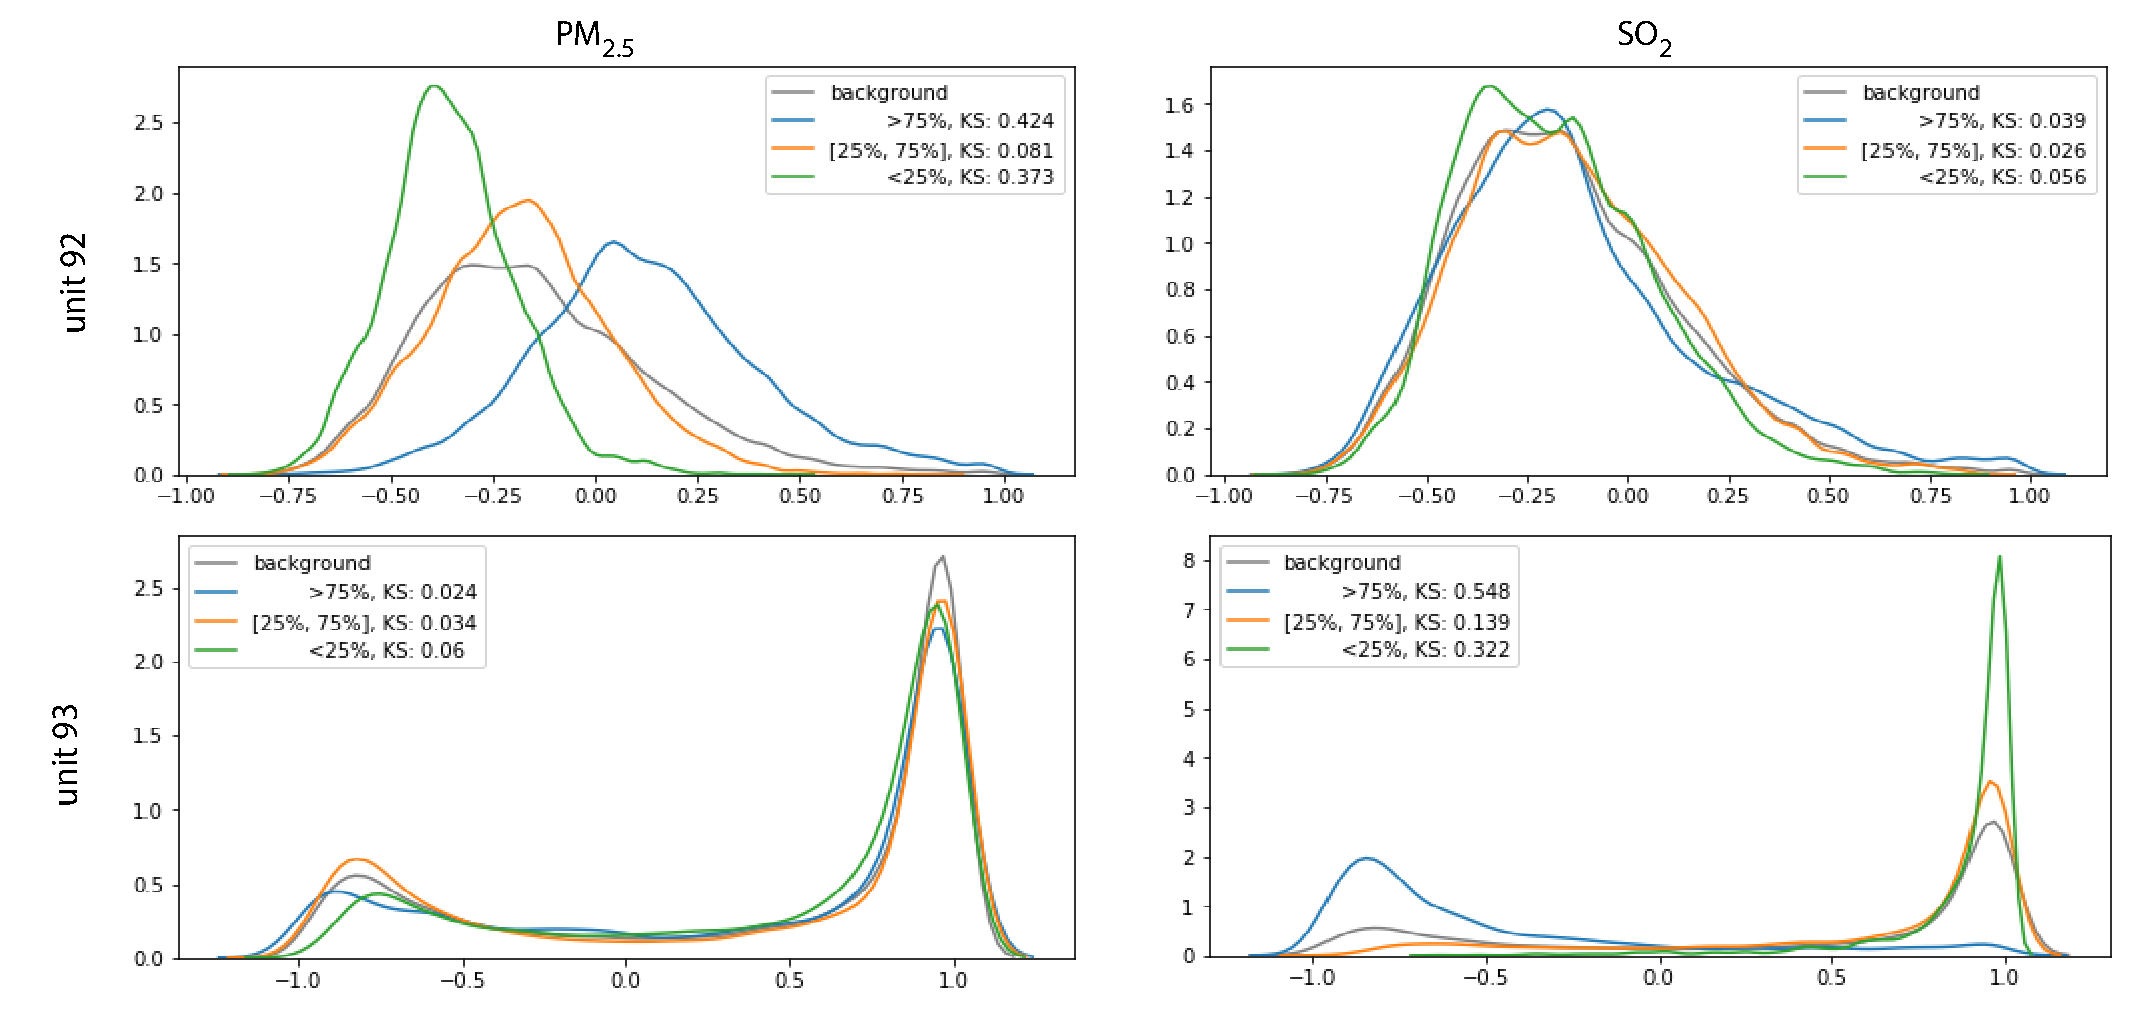
\includegraphics[width=0.45\textwidth]{pictures/unit_response_kdeplot.pdf}
	\vspace{-3mm}
	\caption{Response of hidden unit to $PM_{2.5}$ and $SO_2$.}
	\label{fig:unit_distribution_subgroup}
	\vspace{-4mm}
\end{figure}


%% reasoning
To measure the response between the hidden unit $h^j$ to specific input feature $x^k$, we partition the test data $X$ into three subdivisions by the value of $x^k$: $sub_{bottom}(x^k) = \{x |x^k < perc_{0.25}(x^k), x \in X \}$;$sub_{middle}(x^k) = \{x |perc_{0.25} < (x^k) < perc_{0.75}(x^k), x \in X \}$ and $sub_{top}(x^k) = \{x |x^k > perc_{0.75}(x^k), x \in X \}$. Where $perc_{val}(x^k)$ is the $val^{th}$ percentiles of $x^k$.

As discussed in Sec.~\ref{section:response_and_activation}, the distribution difference between the background and subdivisions of $x^k$ can be used to measure the response of units to specific input dimension. In summary, we use the maximum KS statistics among all subdivisions to qualify the response:
\begin{equation}
    \label{equation:qualify_response}
    \begin{multlined}
    Resp(h^j, x^k) = max(Dif(O(h^j|sub_{bottom}(x^k), X)), \\ 
    Diff(O(h^j|sub_{media}(x^k), X)), 
    Diff(O(h^j|sub_{top}(x^k), X)))
    \end{multlined}
\end{equation}



% \begin{equation}
%     \begin{multlined}$O(h^j|sub(con))$
%     Resp(u^j, f^k) = max(Dif(sub_{bottom}(x^k), X), \\ Dif(sub_{middle}(x^k), X), Dif(sub_{top}(x^k), X)))
%     \end{multlined}
% \end{equation}

\subsection{Hidden units clustering} \label{section:clustering}
Another major challenge for interpreting RNN models on multi-dimensional sequential data is scalability.
RNN models usually contain hundreds to thousands of hidden units for each layer, which makes it ineffective to display the activation distribution of every hidden unit to users.
To address this challenge, previous work on visual interpretation of machine learning models usually use clustering~\cite{ming2017understanding, liu2017towards} or sampling~\cite{pezzotti2018deepeyes} techniques to reduce the number of visual elements displayed at the same time.
In this work, we choose clustering based methods over sampling as clustering can group hidden units with similar behaviors together, which provides users an summarized view of how RNN models response to certain feature value changes.

We first generate hidden unit embeddings and feature embeddings based on the hidden unit response to different features, 
We define hidden unit embedding $vec_{unit}(h^j) = [Resp(h^j, f^0), Resp(h^j, f^1), ..., Resp(h^j, f^{M-1})]$ where $f^k$ represents different features.
The feature vector $vec_{feature}(f^k) $ is defined as the responses from all hidden units to $f^k$: $vec_{feature}(f^k) = [Resp(h^0, f^k), Resp(h^1, f^k), ..., Resp(h^{N-1}, f^k)]$. 

To generate clusters with high quality, we conduct an experiment to select the best performing clustering algorithm and parameters.
In this experiment, we use ~\textit{Silhouette Coefficient} to measure the clustering quality, where a higher score represents a better clustering result.
Table~\ref{table:cluster_features} shows clustering performance for feature embeddings and Table~\ref{table:cluster_units} shows the hidden unit clustering results.
For both tables, each column represents a clustering algorithm and each row represents the cluster number, which is an input parameter to the clustering algorithms
From the table, we observe that Agglomerative Clustering(\textbf{\textit{AC}}) and K-Means show better performance across different number of clusters.
With the table, our system can automatically choose the clustering algorithms and cluster number.~\todo{?} 
Users can also switch to different clustering algorithms and change the number of clusters based on different domain requirements.
% The choosing of clustering algorithms as well as the parameters is the key issues to generate the high-quality clusters. 
% To generate clusters with high quality, we carefully choose our clustering algorithms as well as the parameters.
% Intuitively, co-clustering method is good choice group the hidden units and input data simultaneously, since it can preserve the relationship between hidden units and input data, such method has been adapted in analyzing of RNN behaviour for NLP tasks\cite{ming2017understanding}.
% However, we conduct an experiment to compare the performance across different clustering methods on our clustering tasks, as shown in table \ref{table:cluster_features} and table\ref{table:cluster_units} where the \textit{Silhouette Coefficient} are used to measure the quality of clustering result.  The range of Silhouettle Coefficient is from -1 to 1 indicating the worst to the best. The first columns \textit{\textbf{N}} is the number of clusters. With the table we notice that the Spectral Co-clustering(\textbf{\textit{SCoC}}) have the worst performance for both feature and unit clustering, while Agglomerative Clustering(\textbf{\textit{AC}}) and KMeans have better performance across different number of clustering. With the table, our system can automatically choose the clustering algorithms and cluster number. Notice that for the same algorithms, the performance are slightly changed across different cluster number, our system also visualize the tables and allow end users to select the algorithms and clustering number based on their requirement. 

% |p{2cm}|p{2cm}|
% \begin{tabular}{|c c c c c c c|} 
% \begin{table}[h!]
% \centering
% \vspace{-0.2cm}
% \begin{tabular}{|p{0.2cm}|p{1cm}|p{1cm}|p{1cm}|p{1cm}|p{1cm}|p{1cm}|} 
%  \hline
%  N & AC & KMeans & AP & Birch & SC & SCoC\\ [0.5ex] 
%  \hline
%     8&0.324&0.329&0.305&0.273&0.333&0.273\\ 
%     9&0.336&0.326&0.305&0.288&0.340&0.269\\ 
%     10&0.321&0.337&0.305&0.314&0.335&0.271\\ 
%     11&0.330&0.340&0.305&0.314&0.346&0.280\\ 
%     12&0.339&0.349&0.305&0.311&0.353&0.278\\ 
%     13&0.338&0.343&0.305&0.309&0.347&0.259\\ 
%     14&0.339&0.340&0.305&0.306&0.327&0.263\\ 
%     15&0.343&0.333&0.305&0.311&0.319&0.251\\ 
%     16&0.343&0.336&0.305&0.281&0.321&0.246\\ 
%     17&0.339&0.333&0.305&0.278&0.318&0.298\\ 
%     18&0.333&0.340&0.305&0.282&0.316&0.283\\ 
%     19&0.334&0.328&0.305&0.286&0.310&0.266\\ [1ex] 
% \hline
% \end{tabular}
% \\ [1ex] 
% \caption{Feature clustering performance across different clustering algorithms. AC: Agglomerative Clustering, Affinity Propagation, SC: Spectral Clustering, SCoC: Spectral Co-clustering}
% \label{table:cluster_features}
% \end{table}

% \begin{table}[h!]
% \centering
% \vspace{-0.2cm}
% \begin{tabular}{|p{0.2cm}|p{1cm}|p{1cm}|p{1cm}|p{1cm}|p{1cm}|p{1cm}|} 
%  \hline
%  N & AC & KMeans & AP & Birch & SC & SCoC\\ [0.5ex] 
%  \hline
%     8&0.120&0.111&0.089&0.117&0.107&0.014\\
%     9&0.128&0.118&0.089&0.112&0.108&0.002\\
%     10&0.131&0.114&0.089&0.121&0.117&-0.006\\
%     11&0.127&0.121&0.089&0.102&0.120&-0.015\\
%     12&0.126&0.112&0.089&0.106&0.116&-0.019\\
%     13&0.127&0.106&0.089&0.109&0.114&-0.052\\
%     14&0.130&0.108&0.089&0.108&0.099&-0.034\\
%     15&0.106&0.108&0.089&0.114&0.102&-0.064\\
%     16&0.101&0.099&0.089&0.114&0.054&-0.080\\
%     17&0.104&0.085&0.089&0.111&0.084&-0.091\\
%     18&0.106&0.101&0.089&0.113&0.084&-0.068\\
%     19&0.108&0.099&0.089&0.115&0.085&-0.096\\[1ex] 
% \hline
% \end{tabular}
% \\ [1ex] 
% \caption{Units clustering performance across different clustering algorithms. AC: Agglomerative Clustering, Affinity Propagation, SC: Spectral Clustering, SCoC: Spectral Co-clustering}
% \label{table:cluster_units}
% \end{table}



\begin{figure}[t]
	\centering
	\includegraphics[width=0.45\textwidth]{pictures/cluster_result.pdf}
	\vspace{-3mm}
	\caption{Cluster score}
	\label{fig:unit_distribution_subgroup}
	\vspace{-4mm}
\end{figure}



The clustering results can be modeled as bipartite graph $G = (V_h, V_x, E)$, where $V_h$ is the unit cluster set and $V_x$ is the input dimension cluster set. 
$E$ indicates the weighted edge set between unit clusters and input dimension clusters with the weight of $E_{v,w} = \displaystyle\sum_{h^k \in v}\displaystyle\sum_{x^j \in w}Resp(h^k, x^j)$ where $v \in V$ and $w \in V_x$. 
This bipartite graph of features and hidden units can help users understand the information captured by different hidden unit clusters by examining which feature clusters have strong relations with them.

% In addition, it also provides an overview and alleviate the cognitive burden when explore the relationship between hidden units and features.

\subsection{\QM{Feature importance}}

Inspired by the the back-propagation in machine learning, we conduct the sequence level analysis based on local gradient which is used to present the word saliency in NLP tasks\cite{li2015visualizing}. Given a hidden unit $h^j_t$ which takes previous hidden units $h_{t-1} = [h^0_{t-1},h^1_{t-1},...,h^{N-1}_{t-1}]$ and $x_t = [x^0_t, x^1_t,...,x^{M-1}_t]$ as input, we are able to calculate the local gradient of any $h^j_{t-1}$ or $x^j_t$  with respect to the $h^j_t$:

\begin{equation}
    \label{equation:gradient}
    \begin{multlined}
    w(h^j_t, e) = \frac{\partial(h^j_t)}{\partial(e)}|_e, e \in h_{t-1} \cup x_t
    \end{multlined}
\end{equation}

The element $e$ with larger absolute gradient indicates has a larger influence to the unit output. However, with a given hidden states $h_t$, the total number of gradients is $N \times(N+M)$ which brings difficulty to show the overview of the relationships. To address this challenge, we leverage the clustering get from section \ref{section:clustering}. The aggregated gradient between units cluster $H_t^l$ and $E_t$ are the sum of absolute local gradient between the any hidden unit $h_t^k \in H_t^l$ and element $e \in E_t$:

\begin{equation}
    \label{equation:gradient}
    \begin{multlined}
    w(H_t^l, E^k_t) =\displaystyle\sum_{h^j_t \in H_t^l}\displaystyle\sum_{e^k \in E_t}|w(h^j_t, e^k)|
 \end{multlined}
\end{equation}
